\section{Características do material didático elaborado}\label{sec-caracteristicas}

Após a leitura dos conceitos teóricos explicitados e a conclusão do
curso oferecido pelo CAED, a equipe passou à elaboração do material
didático, levando em consideração o fato de que os alunos inscritos eram
completamente iniciantes ou falso-iniciantes em língua francesa. O
primeiro passo foi, então, recuperar o desenho didático criado no curso
do CAED e preencher a distribuição de conteúdos no sumário do curso,
conforme mostraremos exemplo na \Cref{tab-02}. Os conteúdos foram
distribuídos em três unidades, cada qual com três lições, de maneira a
desenvolver de maneira sistemática as capacidades de linguagem dos
alunos. Em um breve panorama geral, a unidade 0, intitulada
\emph{premiers contacts} (\enquote{primeiros contatos}), teve por objetivo
propor aos alunos identificar a língua francesa em meio a outras
línguas, mapear as palavras de origem francesa em português, reproduzir
a pronúncia de palavras em francês a partir do alfabeto francês, ensinar
os alunos a contar, ou seja, alguns dos elementos básicos iniciais para
o aprendizado de uma língua. A unidade 1, intitulada \emph{bonjour}
(\enquote{olá}), apresentou aos alunos as expressões linguísticas usadas em
francês para se cumprimentar, despedir-se, apresentar-se, informar sua
nacionalidade, sua profissão, levando-os a identificar os tipos de
relação (formais ou informais) em diferentes situações sociais. Por fim,
a unidade 2, intitulada \emph{itinéraires} (\enquote{itinerários}), buscou
colocar os alunos em contato com a cidade em que poderiam morar,
ensinando-os a se localizar, a pedir informações na rua, a descrever de
maneira simples sua cidade, a dizer se gostavam ou não do lugar, entre
outros.

Adotando sempre um gênero textual, oral ou escrito, como ponto de
partida (texto para escuta ou leitura) e como ponto de chegada (texto
para produção, oral ou escrita), cada lição organizou-se em cinco
seções, a saber: \begin{enumerate*}[label=\alph*)]
	\item \emph{découvertes} (\enquote{descobertas});
	\item \emph{étude du genre textuel} (\enquote{estudo do gênero textual});
	\item \emph{focus langue} (\enquote{foco na língua});
	\item \emph{production orale} (\enquote{produção oral});
	\item \emph{production écrite} (\enquote{produção escrita}).
\end{enumerate*}

Todos os conteúdos propostos no curso, tanto comunicativos quanto linguísticos, estavam de
acordo com os descritores de proficiência estruturados no nível A1 do Quadro Europeu Comum de Referência para as Línguas \cite{conselho_da_europa_quadro_2001}.

A título de exemplo, faremos algumas considerações a respeito da lição 3
da unidade 2 do curso (após 36 horas de trabalho), por julgarmos que se
trata do momento em que os alunos, já tendo adquirido as ferramentas
básicas iniciais da língua, participaram com mais desenvoltura do curso.
Buscaremos mostrar, ainda, como se deu a relação entre as atividades
propostas o aprendizado do francês por intermédio da plataforma Moodle e
o suposto desenvolvimento das capacidades de linguagem previstos em
nossos objetivos. Apresentaremos, primeiramente, o sumário da lição (\Cref{tab-02}.

\begin{table}[htpb]
\centering
\begin{threeparttable}
\caption{Sumário da lição 3 (unidade 2).}
\label{tbl-tabela-01}
\begin{tabular}{*{5}{>{\raggedright\arraybackslash}p{2.5cm}}}
\toprule 
Gênero textual prioritário / Domínio social de comunicação / Aspectos tipológicos  &
Objetivos comunicativos &
Objetivos linguísticos &
Aspectos socioculturais &
Ferramentas do Moodle \\
\midrule
- Diálogo entre duas pessoas na rua. 
\newline
Instruções e prescrições.
Descrever ações. Regulação mútua de comportamentos. &
- Compreender e explicar um itinerário. \newline
- Nomear e localizar um lugar. &
- Imperativo.\newline
- Verbo prendre (presente).\newline
- Preposições de lugar.\newline
- Vocabulário: a cidade (comércios, monumentos).
&
- Cidades francófonas (Paris). 
&
- Questionário \newline
- Atividades\newline
- Tarefa\newline
- Rótulo\newline
- URL\newline
- Arquivo \\
\bottomrule
\end{tabular}
\source{Elaborado pelo autor.}
%\notes{Se necessário, poderá ser adicionada uma nota ao final da tabela.}
\end{threeparttable}
\end{table}




A lição 3 da unidade 2 tinha como objetivos comunicativos principais
\enquote{pedir informações na rua a respeito de um itinerário} e \enquote{indicar um itinerário a alguém na rua}. O gênero textual prioritário para a realização desta tarefa foi o diálogo, cujo contexto de produção
apontava para sua realização entre duas pessoas na rua. Esse gênero foi
escolhido pelo fato de que, embora seja comum hoje em dia o uso de
aplicativos de mapas em celulares, ainda é muito possível que as pessoas
cheguem em cidades desconhecidas e peçam informações a habitantes locais
sobre direções, principalmente se ainda não tiverem acesso à internet.
Além disso, em uma perspectiva acional, que privilegia a abordagem
comunicativa autêntica por meio de tarefas, momento em que os alunos
poderiam agir em interação, entendemos que o gênero textual diálogo e a
situação de comunicação escolhida (explicar um itinerário) permitiriam
colocar os alunos em situações bastante concretas de uso da linguagem
que eles poderiam vivenciar empiricamente em um contexto francófono.

Após a escolha do gênero, que seria trabalhado tanto como ponto de
partida (atividade de escuta) quanto como ponto de chegada (atividade de
produção oral) na lição, passou-se à fase da elaboração do MDG. Como o
gênero diálogo é bastante difundido no ensino-aprendizagem de línguas,
uma vez que a maioria dos documentos que visam a trabalhar atividades de
escuta o adotam como documento de trabalho, já tínhamos um MDG elaborado
por nós -- ainda sem publicação - para aulas de francês na graduação,
porém, a partir de um contexto de produção diferente. Assim, ao
recuperarmos esse MDG, fizemos algumas adaptações, sobretudo em relação
ao contexto de produção \cite{bronckart_atividade_1999} do gênero diálogo (o
enunciador e seu papel social; o destinatário e seu papel social; o
local social onde o texto foi produzido; o objetivo da interação),
adaptando-o à nossa situação de compreender e explicar um itinerário na
rua. Ao final desta etapa, havíamos mapeado as características
essenciais definidoras do gênero textual escolhido com vistas à sua
transposição didática \cite{chevallard_transposition_1981} em aulas de FLE. Ao fim desta etapa, a equipe se voltou à elaboração das atividades baseadas no MDG
para cada uma das subseções apresentadas, como poderemos descrever a
seguir.

Na seção \emph{découvertes}, início da lição, os alunos foram colocados
em contato com exercícios introdutórios da temática e das atividades
sociais que levam à produção do gênero diálogo, num levantamento sobre
os conhecimentos prévios sobre a situação de produção do gênero e do
tema da unidade, isto é, um primeiro contato com o gênero que deveriam
produzir. Em seguida, dando continuidade à seção anterior, na seção
\emph{étude du genre textuel} os alunos, ao escutarem o vídeo que
apresentava um diálogo na rua, foram expostos a exercícios que tinham
por objetivo fazê-los discutir sobre seu contato com o gênero e com as
práticas sociais que dão origem a ele, por meio de perguntas, tais
quais: quem produziu o texto? Para quem o texto é dirigido? Qual é o
assunto do texto? Qual o objetivo do texto? Onde esse texto foi
produzido? Quando o texto foi produzido? \cite{stutz_construcao_2011}. A
seguir, poderemos observar o exercício proposto pela \Cref{fig-1}.


\begin{figure}[!htbp]
	\centering
	\begin{minipage}{.8\textwidth}
		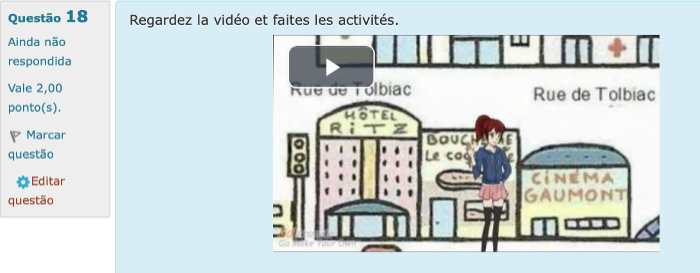
\includegraphics[width=\textwidth]{imagem1.png}
		\caption{Seção \textit{Étude du genre textuel.}}
		\label{fig-1}
		\source{Elaboração própria}
	\end{minipage}
\end{figure}


Nestas duas primeiras etapas, nosso objetivo era desenvolver as
capacidades de ação, por meio da construção de sentido a partir de
representações dos elementos do contexto de produção, da mobilização dos
conteúdos e da escolha do gênero textual \cite{bronckart_atividade_1999}. Dessa
maneira, a fim de mobilizarmos os conhecimentos descritos e atingir de
maneira satisfatória o objetivo da atividade, utilizamos algumas das
funcionalidades oferecidas pela plataforma Moodle. Como se sabe, o
Moodle organiza suas ferramentas em duas categorias: atividades e
recursos. Para o exercício apresentado, foi escolhida a atividade
\enquote{Questionário}, ou seja, um conjunto de questões de vários formatos
diferentes. A ferramenta em questão, bastante utilizada na elaboração do
curso, permite a criação pelo professor de questões de vários formatos,
cabendo ao aluno escolher suas respostas e, em seguida, observar a
correção efetuada pelo sistema a partir de um gabarito previamente
inserido na plataforma pelo professor. No exercício elaborado, a
tipologia de atividade escolhida na plataforma se denomina \enquote{múltipla
escolha}, que permite, também, que o aluno faça mais de uma escolha e
que cada uma das tentativas seja corrigida imediatamente pelo Moodle. Já
o vídeo escolhido para a atividade foi retirado da plataforma YouTube e
inserido no Moodle por meio do recurso \enquote{Rótulo}, que permite a
inserção de textos, imagens e vídeos.

Na terceira subseção, intitulada \emph{focus langue}, buscamos mobilizar
tanto as capacidades discursivas quanto as capacidades
linguístico-discursivas relativas ao gênero textual diálogo. No que diz
respeito às capacidades discursivas, buscamos levar os alunos, por meio
de atividades variadas, a refletirem sobre aspectos organizacionais e
discursivos do gênero, como os tipos de sequência presentes e suas
relações com a situação de produção e os conteúdos temáticos veiculados.
Neste momento, nossa intenção era fazer com que os alunos refletissem
sobre a planificação global do texto, os segmentos organizados de forma
linguística no texto e suas formas de planificação, ou seja, as
sequências \cite{adam_1992,bronckart_atividade_1999}. Algumas de nossas preocupações eram fazer com que os alunos reconhecessem a organização do gênero a partir de seu planejamento geral e compreendessem a função da
organização do conteúdo no gênero diálogo, como ilustra o exercício a
seguir, previsto para que os alunos respondessem às perguntas que já
estavam dadas, relativas ao objetivo comunicativo de indicar um
itinerário na rua. Por meio deste exercício \Cref{fig-2}, os alunos
puderam perceber a forma de organização do conteúdo mobilizado e
refletir sobre a organização do texto.


\begin{figure}[htbp]
	\centering
	\begin{minipage}{0.8\textwidth}
		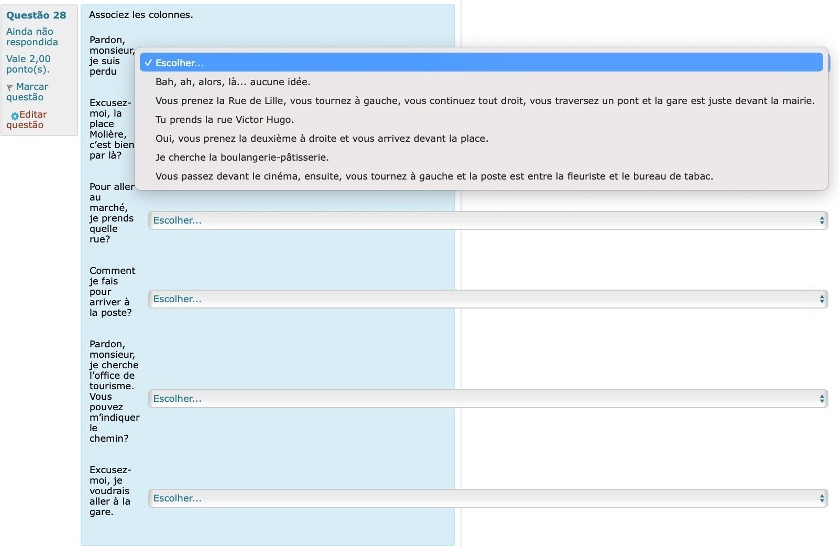
\includegraphics[width=\textwidth]{imagem2.png}
		%Extraído como InkScape
		\caption{Seção \textit{Focus langue.}}
		\label{fig-2}
		\source{Elaboração própria}
	\end{minipage}
\end{figure}

Em relação às capacidades linguístico-discursivas, o objetivo principal
era que os alunos refletissem sobre o estudo da língua francesa, que
elaborassem uma reflexão sobre os elementos linguísticos característicos
do gênero diálogo a partir de uma proposta que partiria da observação à
sistematização da regra. A gramática, neste material, foi considerada
como uma atividade heurística, que permitia ao aluno a reflexão sobre a
língua e a construção de um saber organizado sobre seu funcionamento.
Dessa forma, diferentemente da maioria dos cursos propostos para o
ensino de FLE, os alunos, por meio do método indutivo e mediante a
exposição ao corpus linguístico e a observação de exemplos, puderam
construir as regras e compreender os princípios gramaticais da língua
francesa, o que contribuiu possivelmente para a valorização da
descoberta de regras e das generalizações necessárias naquele estágio,
como comprovaram as produções orais e escritas entregues aos estagiários
para correção.

No exemplo apresentado \Cref{fig-3}, o objetivo é aprender a conjugação do
verbo \emph{prendre} (\enquote{pegar}, \enquote{tomar}), no presente do Indicativo, para, em um contexto de indicar o itinerário na rua, ser capaz de
utilizar, de maneira autônoma, as expressões linguísticas adequadas a
esse fim. A plataforma Moodle permitiu à equipe, também por meio da
ferramenta \enquote{atividades} e \enquote{questionário}, construir de forma
indutiva, como explicado, um exercício por meio da funcionalidade
\enquote{arrastar e soltar na imagem}, em que caberá ao aluno escolher a forma
verbal correspondente, proposta na parte inferior da imagem e, clicando
sobre a forma escolhida, arrastá-la com o mouse até o espaço que
contempla sua resposta. Assim como no exercício descrito anteriormente,
múltiplas respostas são consideradas, mas apenas uma, corrigida
imediatamente pela plataforma Moodle, é considerada adequada.

\begin{figure}[htbp]
	\centering
	\begin{minipage}{0.8\textwidth}
		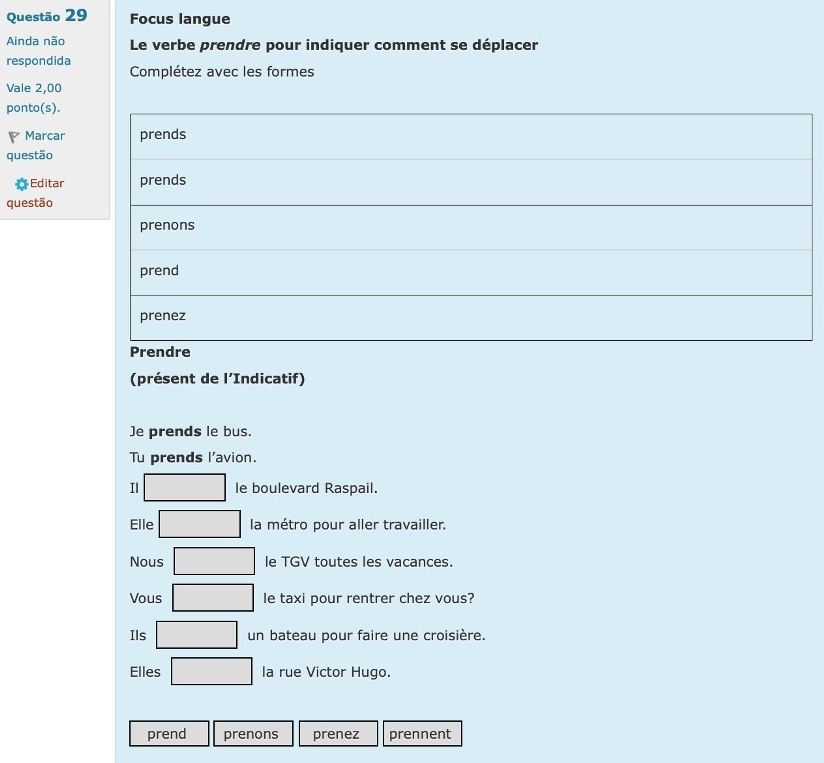
\includegraphics[width=\textwidth]{imagem3.png}
		%Extraído com o InkScape
		\caption{Seção \emph{Focus langue}}
		\label{fig-3}
		\source{Elaboração própria}
	\end{minipage}
\end{figure}


A quarta e última atividade que apresentaremos da lição 3 diz respeito a
uma das propostas de produção oral, sempre associadas ao gênero textual
proposto como texto autêntico de partida para a unidade, ou seja, o
diálogo. A ideia principal, neste momento, é inserir o estudante em uma
situação de comunicação autêntica, o que lhe permite adaptar-se a
situações concretas de uso da linguagem em um contexto francófono,
produzir um novo exemplar do gênero textual e mostrar o que efetivamente
aprendeu após ter realizado as atividades propostas.

Nas três unidades elaboradas, as propostas de produção oral e de
produção escrita permitiram a mobilização das três capacidades de
linguagem juntas, auxiliando, assim, os alunos a desenvolverem não só o
capital linguístico adquirido até então, mas também estratégias de
produção que os conduziam à autonomia em francês. As tarefas de produção
que refletiam situações autênticas em diferentes domínios sociais
(pessoal, público, profissional, etc.) podem ser ilustradas pelo
exercício da \Cref{fig-4}.

\begin{figure}[htbp]
	\centering
	\begin{minipage}{0.8\textwidth}
		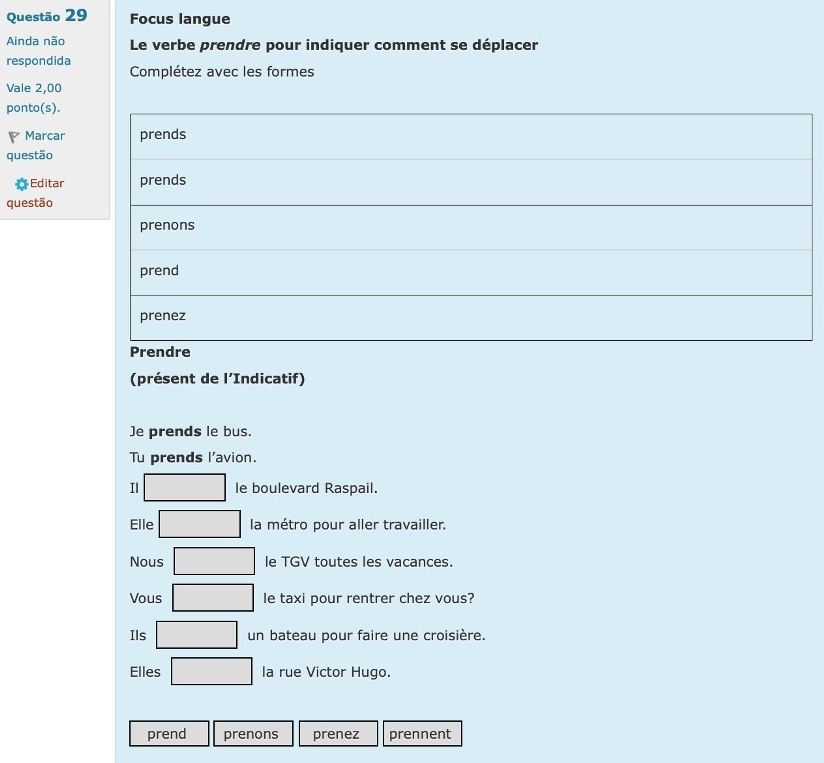
\includegraphics[width=\textwidth]{imagem4.png}
		%extraída usando o InkScape
		\caption{Seção Produção Oral}
		\label{fig-4}
		\source{Elaboração própria}
	\end{minipage}
\end{figure}

Como as aulas eram totalmente assíncronas, as atividades de produção
oral foram adaptadas para refletirem o máximo possível a interação
autêntica em contexto, buscando superar, por vezes, a falta de
espontaneidade decorrente desta modalidade de trabalho. A partir das
explicações no enunciado do exercício, o aluno deveria, inicialmente,
observar um mapa de Paris inserido na plataforma Moodle. Neste mapa,
além da imagem de uma parte da cidade, com suas ruas, pontes,
monumentos, comércios, etc, havia a imagem de duas pessoas que simulavam
um diálogo em uma das ruas. No contexto preparado, uma das pessoas
julgava estar perdida e pedia a outra que lhe explicasse como chegar à
\emph{École des Beaux-Arts} (\enquote{Escola de Belas-Artes}). Ao aluno, no
diálogo, caberia explicar o itinerário, cumprindo, assim, um dos
objetivos comunicativos da lição. Era necessário, portanto, observar o
mapa para se localizar, escutar as frases da pessoa que pedia a
informação (já gravadas pelos estagiários e disponibilizadas no Moodle
em arquivo mp3) e responder a elas, indicando o itinerário demandado a
partir do mapa, buscando simular um diálogo o mais natural possível.
Todas as frases já gravadas pelos estagiários apresentavam, ao seu
final, um sinal sonoro, que indicava o momento em que os alunos deveriam
começar a produzir as suas falas. As falas gravadas pelos alunos, que
completavam o diálogo a partir das frases já gravadas, deveriam ser
enviadas por meio da ferramenta \enquote{Arquivo} da plataforma Moodle, para
que as devidas correções fossem efetuadas pelos estagiários. Após a
correção, um retorno sobre a produção, avaliada em critérios de
adequação ao gênero textual, escolha e pertinência das ideias e dos
argumentos, organização dos conteúdos, coerência e coesão, sintaxe e
vocabulário foi disponibilizado na própria plataforma Moodle, de forma
que o aluno pudesse ter a correção comentada de seu texto e,
principalmente, a possibilidade de autocorreção futura.

Ainda que tenhamos destacado apenas quatro atividades, muitas outras
ferramentas disponibilizadas por Moodle foram igualmente utilizadas pela
equipe, entre elas: a ferramenta \enquote{Fórum}, momento em que uma discussão
assíncrona entre os alunos integrantes da disciplina e também entre
alunos e equipe de professores, sobre conteúdos ministrados, foi
proposta pela equipe; a ferramenta \enquote{Glossário}, em que a inclusão de
palavras pertencentes ao vocabulário relativo ao tema da unidade foi
efetuada; o recurso \enquote{inserir URL}, para que os integrantes da
disciplina pudessem assistir a vídeos oriundos de outras plataformas e
desenvolver sua compreensão oral.

Na última seção, apresentaremos algumas reflexões à guisa de conclusão.
